The following results are based on simulations of the model with parameter
values given in \cref{tab:parameter}. %{\bf (Erich do you remember how we chose
%these numbers?)}\textcolor{red}{No, but clearly some of these need some
%justification. I am guessing a got it from one of the references. I have no
%library access, so it is difficult for me to check the references.}
The grid
size was 101 patches by 101 patches.  The standard error was calculated by
dividing the sample standard deviation by the square root of the total number of
samples. The standard errors were all less than 1\% on average, so will not be
shown due to the small size.

\begin{table}
  \centering
  \begin{tabular}{|l|l|l|l|}
    \hline
    Parameter Description & Symbol & Value &  \\ \hline  \label{parameter}
    Total number of animals & b & 1,000 & fixed  \\ \hline
    Maximum time & $t_{max}$ & 1,200 seconds & fixed \\ \hline
    Fraction of blooms at one time & a & 0.2 & fixed \\ \hline
    Maximum fraction of available flowers & $\eta$ & 0.75 & fixed \\ \hline
    Search radius & r & 1.0 & fixed \\ \hline
    Number of flowers per plant & $\phi$ & 100 & fixed \\ \hline
    Probability of pollination   & $\rho$ & 0.4286 & calculated \\ \hline
    Number of plants & n & 1000 & fixed \\ \hline
    Time spent at each plant & $t_{plant}$ & 100 seconds & fixed \\ \hline
  \end{tabular}
  \caption{Parameter Values}
  \label{tab:parameter}
\end{table}

\begin{figure}
  \begin{center}
  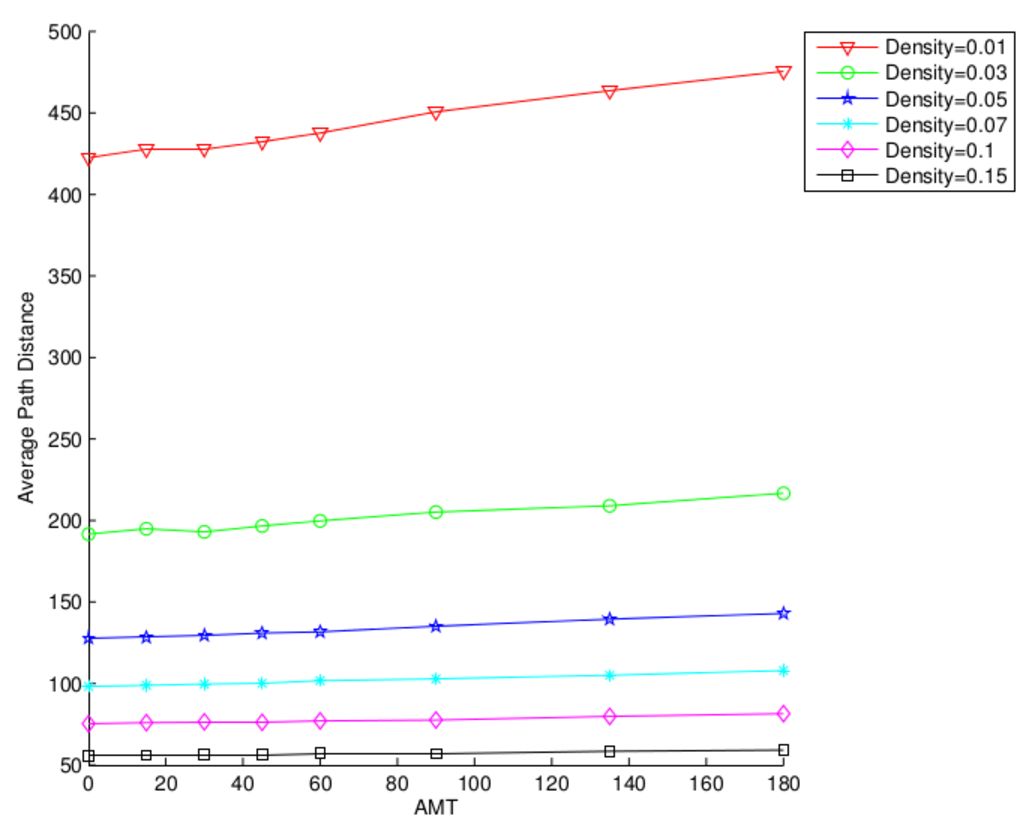
\includegraphics[scale=0.5]{Figures/PathVsAMT.pdf}
  \end{center}
  \caption{\small Average Path Distance vs. Turning Angle for Various Plant
    Densities}
  \label{AvgPathN}
\end{figure}

In \cref{AvgPathN} the average distance traveled for each animal decreases
with increasing density due to higher foraging success.  In this situation the
animals will spend more time on plants since they can find plants more readily
and thus reach their maximum searching time more quickly.  The maximum turning
angle does not have a large effect on on the  average distance in general,
though there is a modest effect at low plant densities where the larger values
increase the average distance due to less success at foraging.

On the other hand, the average maximum distance traveled by animals, see
\cref{AvgMaxDBees}, is affected by both the turning angle and plant density.
As with the average path distance, the maximum distance decreases with higher
density for the same reason that this decreases the overall travel time for the
animals since they spend more time on plants.  In this case due to the movement
patterns the maximum turning angle has a large effect on maximum distance
traveled especially at lower densities.  As the maximum angle decreases the
animals are moving in a more highly correlated random walk and are more likely
to travel directly away from their starting points increasing the maximum
distance traveled.

In particular at high density for a moderately correlated random walk
$(AMT=90^{\circ})$ there is an increase of over 30\% for the maximum distance
over the purely random walk, and for a highly correlated random walk
$(AMT=45^{\circ})$ there is an increase of 67\%.  At lower densities this is
more pronounced.  There is an increase in the maximum distance traveled by 62\%
and 160\% over the purely random walk by a moderately and highly correlated
random walks, respectively. These differences can have important consequences on
the overall genetic diversity for the plants, and shows that biotic dispersal
has a greater potential for long range pollination over abiotic
dispersal.

\begin{figure}
  \begin{center}
  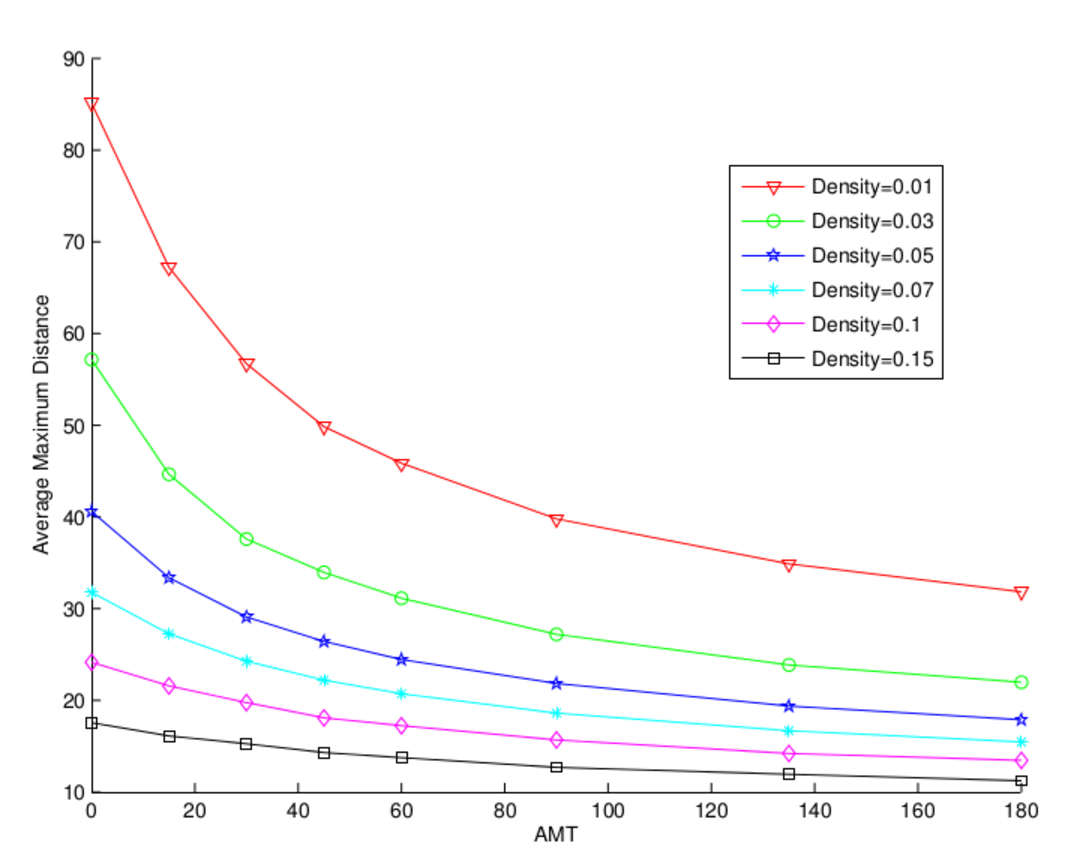
\includegraphics[scale=0.5]{Figures/MaxDVsAMT.pdf}
  \end{center}
  \caption{\small Average Maximum Distance vs. Turning Angle for Various Plant Densities}
  \label{AvgMaxDBees}
\end{figure}

We see this potential in \cref{AvgDist} where, like the average maximum
distance, the average pollination distance increases with stronger correlation
and at lower density.  At high densities the effects of correlation are smaller.
This is due to the fact that when pollinators plants they leave each
plant in a random direction, and so as plant density increases the number of
plant visits increases, which consequently has them behave more like a
purely random walk.  It is also the case, as with the average maximum distance,
as the maximum angle decreases and the correlation strengthens, the animal is
likely to travel farther from its initial position, which allows for longer
pollination distances.

At low densities there is an increase in the average pollination distance of
36\% and 96\% over a purely random walk for a moderately and highly correlated
random walk, respectively.  At high density the increases are 29\% and 65\%,
respectively.  These increases will have significant impact on the overall gene
flow of the plant species.

\begin{figure}
  \begin{center}
  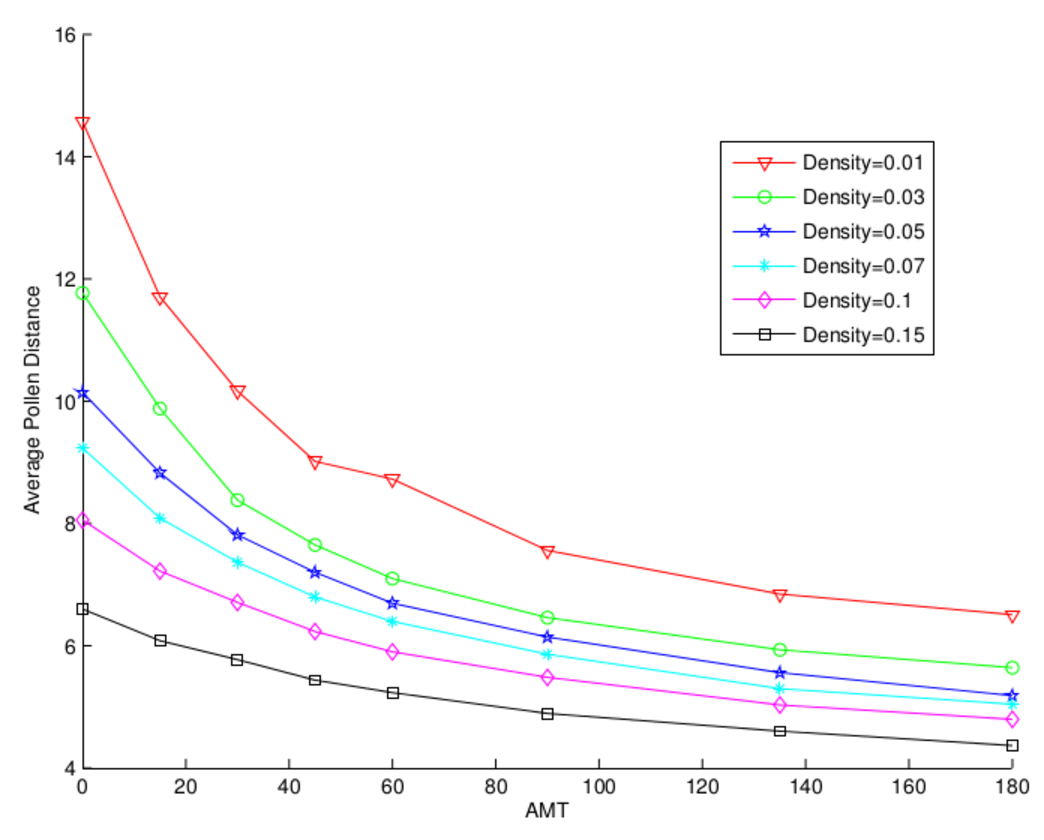
\includegraphics[scale=0.5]{Figures/PollenDVsAMT.pdf}
  \end{center}
  \caption{\small Average Pollination Distance vs. Turning Angle for Various Plant Densities}
  \label{AvgDist}
\end{figure}

These increases are also observed for the maximum pollination distance.  For low
plant densities the average maximum pollination distance increases by 53\% for
moderately correlated random walks over purely random walks, and 148\% for
highly correlated random walks.  Additionally, for high plant densities these
increases are 44\% and 96\% for moderately and highly correlated random walks
over purely random walks, respectively.  Since these are average values there is
clearly a potential for much greater range of pollen dispersal and genetic
variation with biotic dispersal over abiotic dispersal.

\begin{figure}
  \begin{center}
  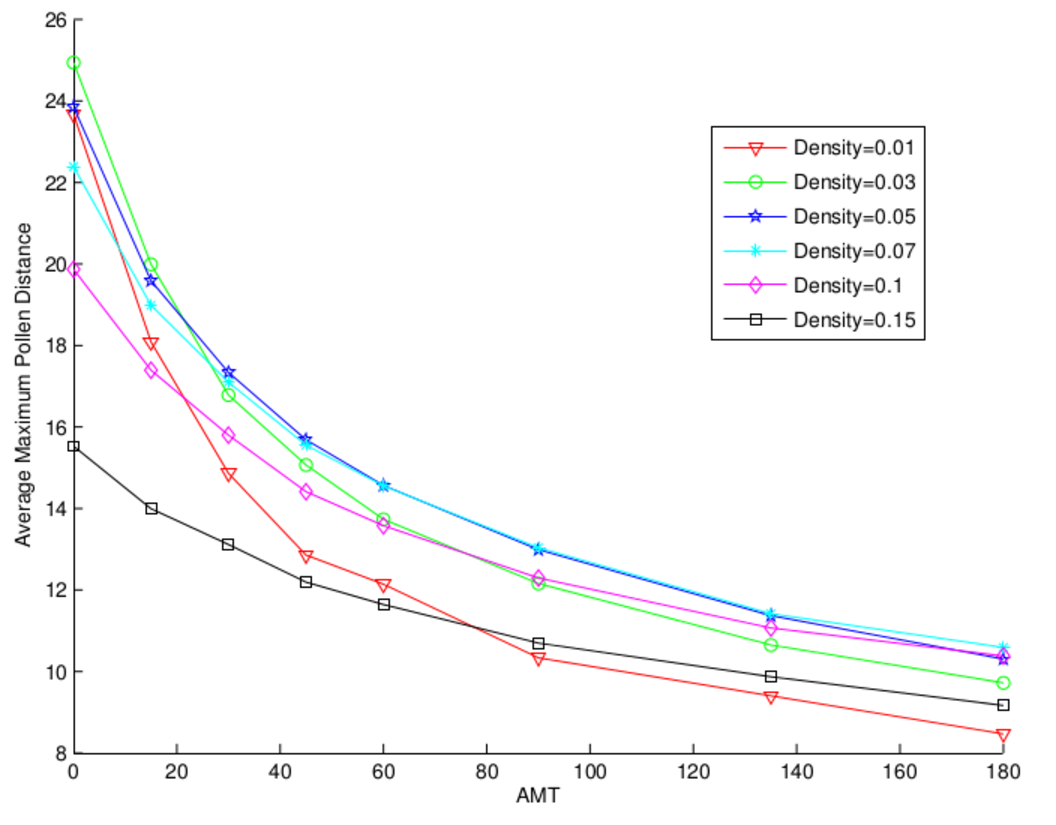
\includegraphics[scale=0.5]{Figures/MaxPollenVsAMT.pdf}
  \end{center}
  \caption{\small Average Maximum Pollination Distance vs. Turning Angle for Various Plant Densities}
  \label{AvgMaxDTreesN}
\end{figure}

Plant density affects the maximum pollination distance in a more complex
fashion.  The higher the density the more gradual the decrease is in the maximum
pollination distance as the maximum turning angle increases.  Whereas, at lower
densities this decrease is much larger.  This is due to the fact at lower
densities pollination occurs less frequently with a larger variability of
maximum pollination distances.

\begin{figure}
  \begin{center}
  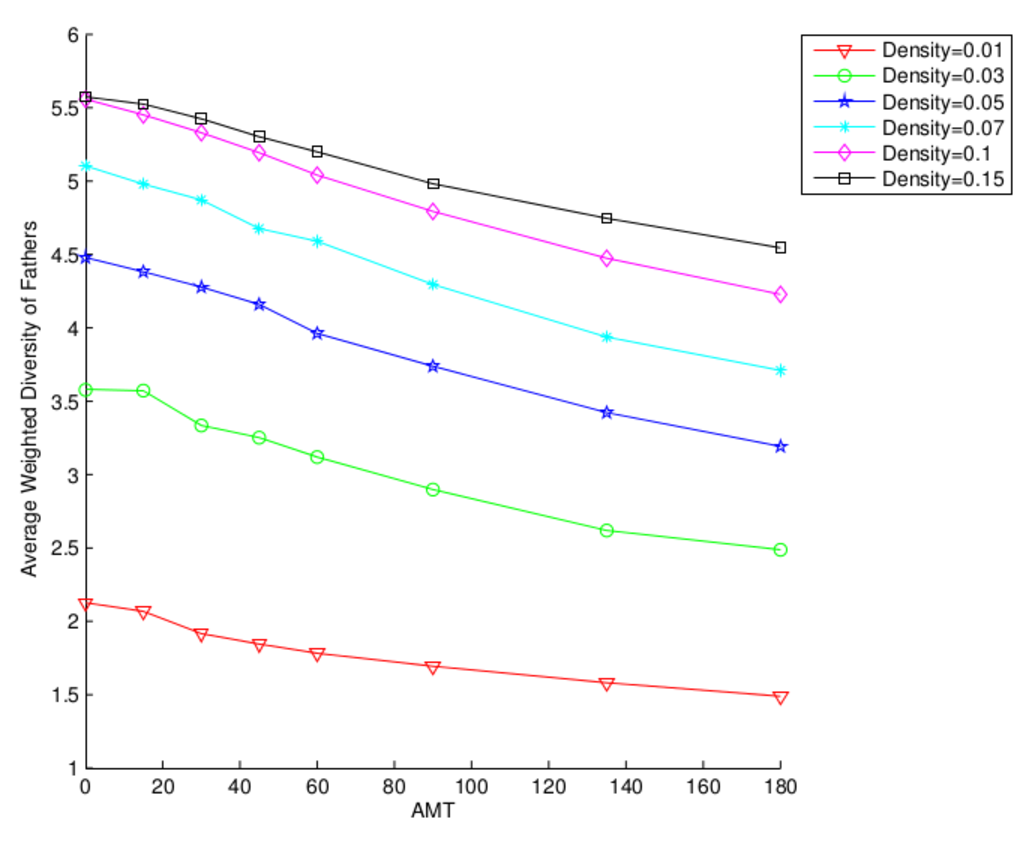
\includegraphics[scale=0.5]{Figures/WDFvsAMT.pdf}
  \end{center}
  \caption{\small Average Weighted Diversity of Fathers vs. Turning Angle for Various Plant Densities}
  \label{EFathers}
\end{figure}

In general there is a small decrease in the average weighted diversity of
fathers as the maximum turning angle increases, see \cref{EFathers}. With
higher maximum turning angles the search patterns tend to be more circular
lowering the overall diversity that a plant will see since pollinators will
visit the same plants more frequently.  On the other hand, by increasing the
density, plants will see an increase in diversity due to the larger amount of
plants near by.  This increase lessens at higher densities due to the limited
foraging time of the pollinators.
